\documentclass{article}
\usepackage[backend=biber,natbib=true,style=alphabetic,maxbibnames=50]{biblatex}
\addbibresource{/home/nqbh/reference/bib.bib}
\usepackage[utf8]{vietnam}
\usepackage{tocloft}
\renewcommand{\cftsecleader}{\cftdotfill{\cftdotsep}}
\usepackage[colorlinks=true,linkcolor=blue,urlcolor=red,citecolor=magenta]{hyperref}
\usepackage{amsmath,amssymb,amsthm,float,graphicx,mathtools}
\allowdisplaybreaks
\newtheorem{assumption}{Assumption}
\newtheorem{baitoan}{}
\newtheorem{cauhoi}{Câu hỏi}
\newtheorem{conjecture}{Conjecture}
\newtheorem{corollary}{Corollary}
\newtheorem{dangtoan}{Dạng toán}
\newtheorem{definition}{Definition}
\newtheorem{dinhly}{Định lý}
\newtheorem{dinhnghia}{Định nghĩa}
\newtheorem{example}{Example}
\newtheorem{ghichu}{Ghi chú}
\newtheorem{hequa}{Hệ quả}
\newtheorem{hypothesis}{Hypothesis}
\newtheorem{lemma}{Lemma}
\newtheorem{luuy}{Lưu ý}
\newtheorem{nhanxet}{Nhận xét}
\newtheorem{notation}{Notation}
\newtheorem{note}{Note}
\newtheorem{principle}{Principle}
\newtheorem{problem}{Problem}
\newtheorem{proposition}{Proposition}
\newtheorem{question}{Question}
\newtheorem{remark}{Remark}
\newtheorem{theorem}{Theorem}
\newtheorem{vidu}{Ví dụ}
\usepackage[left=1cm,right=1cm,top=5mm,bottom=5mm,footskip=4mm]{geometry}
\def\labelitemii{$\circ$}
\DeclareRobustCommand{\divby}{%
	\mathrel{\vbox{\baselineskip.65ex\lineskiplimit0pt\hbox{.}\hbox{.}\hbox{.}}}%
}

\title{Problem: Application of Derivative to Survey \& Draw Graph of Functions\\Bài Tập: Ứng Dụng Đạo Hàm Để Khảo Sát \& Vẽ Đồ Thị của Hàm Số}
\author{Nguyễn Quản Bá Hồng\footnote{Independent Researcher, Ben Tre City, Vietnam\\e-mail: \texttt{nguyenquanbahong@gmail.com}; website: \url{https://nqbh.github.io}.}}
\date{\today}

\begin{document}
\maketitle
\tableofcontents

%------------------------------------------------------------------------------%

\section{Tính Đơn Điệu của Hàm Số}

%------------------------------------------------------------------------------%

\begin{baitoan}[\cite{SGK_Toan_12_giai_tich_nang_cao}, Ví dụ 1, p. 5]
	Chứng minh hàm số $f(x) = \sqrt{1 - x^2}$ nghịch biến trên đoạn $[0,1]$.
\end{baitoan}

\begin{baitoan}[\cite{SGK_Toan_12_giai_tich_nang_cao}, Ví dụ 2, p. 6]
	Xét chiều biến thiên của hàm số $y = x + \frac{4}{x}$.
\end{baitoan}

\begin{baitoan}[\cite{SGK_Toan_12_giai_tich_nang_cao}, H1, p. 6]
	Xét chiều biến thiên của hàm số $y = \frac{1}{3}x^3 - \frac{3}{2}x^2 + 2x - 3$.
\end{baitoan}

\begin{baitoan}[\cite{SGK_Toan_12_giai_tich_nang_cao}, Ví dụ 3, p. 6]
	Xét chiều biến thiên của hàm số $y = \frac{4}{3}x^3 - 2x^2 + x - 3$.
\end{baitoan}

\begin{baitoan}[\cite{SGK_Toan_12_giai_tich_nang_cao}, H2, p. 7]
	Xét chiều biến thiên của hàm số $y = 2x^5 + 5x^4 + \frac{10}{3}x^3 - \frac{7}{3}$.
\end{baitoan}

\begin{baitoan}[\cite{SGK_Toan_12_giai_tich_nang_cao}, 1., p. 7]
	Xét chiều biến thiên của hàm số: (a) $y = 2x^3 + 3x^2 + 1$. (b) $y = x^3 - 2x^2 + x + 1$. (c) $y = x + \frac{3}{x}$. (d) $y = x - \frac{2}{x}$. (e) $y = x^4 - 2x^2 - 5$. (f) $y = \sqrt{4 - x^2}$.
\end{baitoan}

\begin{baitoan}[\cite{SGK_Toan_12_giai_tich_nang_cao}, 2., p. 7]
	Chứng minh: (a) Hàm số $y = \dfrac{x - 2}{x + 2}$ đồng biến trên mỗi khoảng xác định của nó. (b) Hàm số $y = \dfrac{-x^2 - 2x + 3}{x + 1}$ nghịch biến trên mỗi khoảng xác định của nó.
\end{baitoan}

\begin{baitoan}[\cite{SGK_Toan_12_giai_tich_nang_cao}, 3., p. 8]
	Chứng minh các hàm số sau đây đồng biến trên $\mathbb{R}$: (a) $f(x) = x^3 - 6x^2 + 17x + 4$. (b) $f(x) = x^3 + x - \cos x - 4$.
\end{baitoan}

\begin{baitoan}[\cite{SGK_Toan_12_giai_tich_nang_cao}, 4., p. 8]
	Với giá trị nào của $a$ hàm số $y = ax - x^3$ nghịch biến trên $\mathbb{R}$?
\end{baitoan}

\begin{baitoan}[\cite{SGK_Toan_12_giai_tich_nang_cao}, 5., p. 8]
	Tìm các giá trị của tham số $a$ để hàm số $f(x) = \frac{1}{3}x^3 + ax^2 + 4x + 3$ đồng biến trên $\mathbb{R}$.
\end{baitoan}

\begin{baitoan}[\cite{SGK_Toan_12_giai_tich_nang_cao}, 6., p. 8]
	Xét chiều biến thiên của hàm số: (a) $y = \frac{1}{3}x^3 - 2x^2 + 4x - 5$. (b) $y = -\frac{4}{3}x^3 + 6x^2 - 9x - \frac{2}{3}$. (c) $y = \dfrac{x^2 - 8x + 9}{x - 5}$. (d) $y = \sqrt{2x - x^2}$. (e) $y = \sqrt{x^2 - 2x + 3}$. (f) $y = \dfrac{1}{x + 1} - 2x$.
\end{baitoan}

\begin{baitoan}[\cite{SGK_Toan_12_giai_tich_nang_cao}, 7., p. 8]
	Chứng minh hàm số $f(x) = \cos2x - 2x + 3$ nghịch biến trên $\mathbb{R}$.
\end{baitoan}

\begin{baitoan}[\cite{SGK_Toan_12_giai_tich_nang_cao}, 8., pp. 8--9]
	Chứng minh bất đẳng thức: (a) $\sin x < x$, $\forall x\in\mathbb{R}$, $x > 0$; $\sin x > x$, $\forall x\in\mathbb{R}$, $x < 0$. (b) $\cos x > 1 - \frac{x^2}{2}$, $\forall x\in\mathbb{R}$, $x\ne0$. (c) $\sin x > x - \frac{x^3}{6}$, $\forall x\in\mathbb{R}$, $x > 0$; $\sin x < x - \frac{x^3}{6}$, $\forall x\in\mathbb{R}$, $x < 0$.
\end{baitoan}

\begin{baitoan}[\cite{SGK_Toan_12_giai_tich_nang_cao}, 9., p. 9]
	Chứng minh: $\sin x + \tan x > 2x$, $\forall x\in\left(0,\frac{\pi}{2}\right)$.
\end{baitoan}

\begin{baitoan}[\cite{SGK_Toan_12_giai_tich_nang_cao}, 10., p. 9]
	Số dân của 1 thị trấn sau $t$ năm kể từ năm 1970 được ước tính bởi công thức $f(t) = \dfrac{26t + 10}{t + 5}$ ($f(t)$ được tính bằng nghìn người). (a) Tính số dân của thị trấn vào năm 1980 \& năm 1995. (b) Xem $f$ là 1 hàm số xác định trên nửa khoảng $[0,+\infty)$. Tìm $f'$ \& xét chiều biến thiên của hàm số $f$ trên nửa khoảng $[0,+\infty)$. (c) Đạo hàm của hàm số $f$ biểu thị tốc độ tăng dân số của thị trấn (tính bằng nghìn người{\tt/}năm). Tính tốc độ tăng dân số vào năm 1990 \& năm 2008 của thị trấn. Vào năm nào thì tốc độ tăng dân số là $0.125$ nghìn người{\tt/}năm?
\end{baitoan}

%------------------------------------------------------------------------------%

\section{Cực Trị của Hàm Số}

\begin{baitoan}[\cite{SGK_Toan_12_giai_tich_nang_cao}, Ví dụ 1, p. 14]
	Tìm cực trị của hàm số $f(x) = \frac{1}{3}x^3 - x^2 - 3x + \frac{4}{3}$.
\end{baitoan}

\begin{baitoan}[\cite{SGK_Toan_12_giai_tich_nang_cao}, H1, p. 14]
	Tìm cực trị của hàm số $f(x) = x + \frac{4}{x} - 3$.
\end{baitoan}

\begin{baitoan}[\cite{SGK_Toan_12_giai_tich_nang_cao}, Ví dụ 2, p. 14]
	Tìm cực trị của hàm số $f(x) = |x|$.
\end{baitoan}

\begin{baitoan}[\cite{SGK_Toan_12_giai_tich_nang_cao}, Ví dụ 3, p. 16]
	Tìm cực trị của hàm số $f(x) = \frac{1}{3}x^3 - x^2 - 3x + \frac{4}{3}$.
\end{baitoan}

\begin{baitoan}[\cite{SGK_Toan_12_giai_tich_nang_cao}, H2, p. 16]
	Tìm cực trị của hàm số $f(x) = 2\sin2x - 3$.
\end{baitoan}

\begin{baitoan}[\cite{SGK_Toan_12_giai_tich_nang_cao}, 11., pp. 16--17]
	Tìm cực trị của hàm số: (a) $f(x) = \frac{1}{3}x^3 + 2x^2 + 3x - 1$. (b) $f(x) = \frac{1}{3}x^3 - x^2 + 2x - 10$. (c) $f(x) = x + \frac{1}{x}$. (d) $f(x) = |x|(x + 2)$. (e) $f(x) = \frac{1}{5}x^5 - \frac{1}{3}x^3 + 2$. (f) $f(x) = \dfrac{x^2 - 3x + 3}{x - 1}$.
\end{baitoan}

\begin{baitoan}[\cite{SGK_Toan_12_giai_tich_nang_cao}, 12., p. 17]
	Tìm cực trị của hàm số: (a) $y = x\sqrt{4 - x^2}$. (b) $y = \sqrt{8 - x^2}$. (c) $y = x - \sin2x + 2$. (d) $y = 3 - 2\cos x - \cos2x$.
\end{baitoan}

\begin{baitoan}[\cite{SGK_Toan_12_giai_tich_nang_cao}, 13., p. 17]
	Tìm 4 hệ số $a,b,c,d\in\mathbb{R}$ của hàm số $f(x) = ax^3 + bx^2 + cx + d$ sao cho hàm số $f$ đạt cực tiểu tại điểm $x = 0$, $f(0) = 0$, \& đạt cực đại tại điểm $x = 1$, $f(1) = 1$.
\end{baitoan}

\begin{baitoan}[\cite{SGK_Toan_12_giai_tich_nang_cao}, 14., p. 17]
	Xác định 3 hệ số $a,b,c\in\mathbb{R}$ sao cho hàm số $f(x) = x^3 + ax^2 + bx + c$ đạt cực trị bằng $0$ tại điểm $x = -2$ \& đồ thị của hàm số đi qua điểm $A(1,0)$.
\end{baitoan}

\begin{baitoan}[\cite{SGK_Toan_12_giai_tich_nang_cao}, 15., p. 17]
	Chứng minh với mọi giá trị của $m$, hàm số $y = \dfrac{x^2 - m(m + 1)x + m^3 + 1}{x - m}$ luôn có cực đại \& cực tiểu.
\end{baitoan}

%------------------------------------------------------------------------------%

\section{GTLN \& GTNN của Hàm Số}

\begin{baitoan}[\cite{SGK_Toan_12_giai_tich_nang_cao}, Ví dụ 1, p. 18]
	Tìm {\rm GTLN, GTNN} của hàm số $f(x) = \sqrt{4 - x^2}$.
\end{baitoan}

\begin{baitoan}[\cite{SGK_Toan_12_giai_tich_nang_cao}, Ví dụ 2, p. 19]
	Tìm {\rm GTLN, GTNN} của hàm số $f(x) = x^3 - 3x + 3$ trên đoạn $\left[-3,\frac{3}{2}\right]$.
\end{baitoan}

\begin{baitoan}[\cite{SGK_Toan_12_giai_tich_nang_cao}, H, p. 19]
	Tìm {\rm GTLN, GTNN} của hàm số $f(x) = x + \dfrac{1}{x - 1}$ trên khoảng $(1,+\infty)$.
\end{baitoan}

\begin{baitoan}[\cite{SGK_Toan_12_giai_tich_nang_cao}, Ví dụ 3, p. 20]
	1 hộp không nắp được làm từ 1 mảnh các tông theo mẫu như hình:
	\begin{figure}[H]
		\centering
		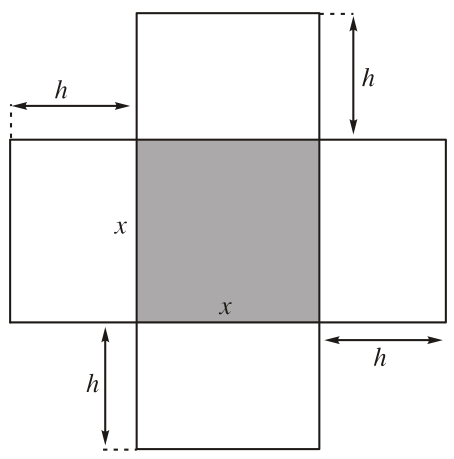
\includegraphics[scale=.25]{hop_khong_nap}
	\end{figure}
	\noindent Hộp có đáy là 1 hình vuông cạnh $x$ {\rm cm}, chiều cao là $h$ {\rm cm}, \& có thể tích là $500$ $\rm cm^3$. (a) Biểu diễn $h$ theo $x$. (b) Tìm diện tích $S(x)$ của mảnh các tông theo $x$. (c) Tìm giá trị của $x$ sao cho $S(x)$ nhỏ nhất.
\end{baitoan}

\begin{baitoan}[\cite{SGK_Toan_12_giai_tich_nang_cao}, Ví dụ 4, p. 21]
	Tìm {\rm GTLN, GTNN} của hàm số $f(x) = x^3 - 3x + 3$ trên đoạn $[0,2]$.
\end{baitoan}

\begin{baitoan}[\cite{SGK_Toan_12_giai_tich_nang_cao}, 16., p. 22]
	Tìm {\rm GTLN, GTNN} của hàm số $f(x) = \sin^4x + \cos^4x$.
\end{baitoan}

\begin{baitoan}[\cite{SGK_Toan_12_giai_tich_nang_cao}, 17., p. 22]
	Tìm {\rm GTLN, GTNN} của hàm số: (a) $f(x) = x^2 + 2x - 5$ trên đoạn $[-2,3]$. (b) $f(x) = \frac{1}{3}x^3 + 2x^2 + 3x - 4$ trên đoạn $[-4,0]$. (c) $f(x) = x + \frac{1}{x}$ trên khoảng $(0,+\infty)$. (d) $f(x) = -x^2 + 2x + 4$ trên đoạn $[2,4]$. (e) $f(x) = \dfrac{2x^2 + 5x + 4}{x + 2}$ trên đoạn $[0,1]$. (f) $f(x) = x - \frac{1}{x}$ trên nửa khoảng $(0,2]$.
\end{baitoan}

\begin{baitoan}[\cite{SGK_Toan_12_giai_tich_nang_cao}, 18., p. 22]
	Tìm {\rm GTLN, GTNN} của hàm số: (a) $y = 2\sin^2x + 2\sin x - 1$. (b) $\cos^22x - \sin x\cos x + 4$.
\end{baitoan}

\begin{baitoan}[\cite{SGK_Toan_12_giai_tich_nang_cao}, 19., p. 22]
	Cho $\Delta ABC$ đều cạnh $a$. Dựng 1 hình chữ nhật $MNPQ$ có cạnh $MN$ nằm trên cạnh $BC$, 2 đỉnh $P,Q$ theo thứ tự nằm trên 2 cạnh $AC,AB$ của tam giác. Xác định vị trí của điểm $M$ sao cho hình chữ nhật có diện tích lớn nhất \& tìm {\rm GTLN} đó.
\end{baitoan}

\begin{baitoan}[\cite{SGK_Toan_12_giai_tich_nang_cao}, 20., p. 22]
	Khi nuôi cá thí nghiệm trong hồ, 1 nhà sinh vật học thấy: Nếu trên mỗi đơn vị diện tích của mặt hồ có $n$ con cá thì trung bình mỗi con cá sau 1 vụ cân nặng $P(n) = 480 - 20n$ {\rm g}. Hỏi phải thả bao nhiêu cá trên 1 đơn vị diện tích của mặt hồ để sau 1 vụ thu hoạch được nhiều cá nhất?
\end{baitoan}

\begin{baitoan}[\cite{SGK_Toan_12_giai_tich_nang_cao}, 21., p. 23]
	Tìm cực trị của hàm số: (a) $f(x)  = \dfrac{x}{x^2 + 1}$. (b) $f(x) = \dfrac{x^3}{x + 1}$. (c) $f(x) = \sqrt{5 - x^2}$. (d) $f(x) = x + \sqrt{x^2 - 1}$.
\end{baitoan}

\begin{baitoan}[\cite{SGK_Toan_12_giai_tich_nang_cao}, 22., p. 23]
	Tìm giá trị của $m$ để hàm số $f(x) = \dfrac{x^2 + mx - 1}{x - 1}$ có cực đại \& cực tiểu.
\end{baitoan}

\begin{baitoan}[\cite{SGK_Toan_12_giai_tich_nang_cao}, 23., p. 23]
	Độ giảm huyết áp của 1 bệnh nhân được cho bởi công thức $G(x) = 0.025x^2(30 - x)$, trong đó $x$ là liều lượng thuốc được tiêm cho bệnh nhân ($x$ được tính bằng {\rm mg}). Tính liều lượng thuốc cần tiêm cho bệnh nhân để huyết áp giảm nhiều nhất \& tính độ giảm đó.
\end{baitoan}

\begin{baitoan}[\cite{SGK_Toan_12_giai_tich_nang_cao}, 24., p. 23]
	Cho parabol $(\mathcal{P}):\ y = x^2$ \& điểm $A(-3,0)$. Xác định điểm $M$ thuộc parabol $(\mathcal{P})$ sao cho khoảng cách $AM$ là ngắn nhất \& tìm khoảng cách ngắn nhất đó.
\end{baitoan}

\begin{baitoan}[\cite{SGK_Toan_12_giai_tich_nang_cao}, 25., p. 23]
	1 con cá hồi bơi ngược dòng để vượt 1 khoảng cách là {\rm300 km}. Vận tốc dòng nước là {\rm6 km{\tt/}h}. Nếu vận tốc bơi của cá khi nước đứng yên là $v$ {\rm km{\tt/}h} thì năng lượng tiêu hao của cá trong $t$ giờ được cho bởi công thức $E(v) = cv^3t$, trong đó $c$ là 1 hằng số, $E$ được tính bằng jule. Tìm vận tốc bơi của cá khi nước đứng yên để năng lượng tiêu hao là ít nhất.
\end{baitoan}

\begin{baitoan}[\cite{SGK_Toan_12_giai_tich_nang_cao}, 26., pp. 23--24]
	Sau khi phát hiện 1 bệnh dịch, các chuyên gia y tế ước tính số người nhiễm bệnh kể từ ngày xuất hiện bệnh nhân đầu tiên đến ngày thứ $t$ là $f(t) = 45t^2 - t^3$, $t = 0,1,2,\ldots,25$. Nếu coi $f$ là hàm số xác định trên đoạn $[0,25]$ thì $f'(t)$ được xem là tốc độ truyền bệnh (người{\tt/}ngày) tại thời điểm $t$. (a) Tính tốc độ truyền bệnh vào ngày thứ 5. (b) Xác định ngày mà tốc độ truyền bệnh là lớn nhất \& tính tốc độ đó. (c) Xác định các ngày mà tốc độ truyền bệnh lớn hơn $600$. (d) Xét chiều biến thiên của hàm số $f$ trên đoạn $[0,25]$.
\end{baitoan}

\begin{baitoan}[\cite{SGK_Toan_12_giai_tich_nang_cao}, 27., p. 24]
	Tìm {\rm GTLN, GTNN} của hàm số: (a) $f(x) = \sqrt{3 - 2x}$ trên đoạn $[-3,1]$. (b) $f(x) = x + \sqrt{4 - x^2}$. (c) $f(x) = \sin^4x + \cos^2x + 2$. (d) $f(x) = x - \sin2x$ trên đoạn $\left[-\frac{\pi}{2},\pi\right]$.
\end{baitoan}

\begin{baitoan}[\cite{SGK_Toan_12_giai_tich_nang_cao}, 28., p. 24]
	Trong các hình chữ nhật có chu vi là {\rm40 cm}, xác định hình chữ nhật có diện tích lớn nhất.
\end{baitoan}

%------------------------------------------------------------------------------%

\section{Đồ Thị của Hàm Số \& Phép Tịnh Tiến Hệ Tọa Độ}

\begin{baitoan}[\cite{SGK_Toan_12_giai_tich_nang_cao}, Ví dụ, p. 26]
	Cho đường cong $(\mathcal{C})$ có phương trình: $y = \frac{1}{2}(x - 2)^3 - 1$ \& điểm $I(2,-1)$. (a) Viết công thức chuyển hệ tọa độ trong phép tịnh tiến theo vector $\vec{OI}$ \& viết phương trình của đường cong $(\mathcal{C})$ đối với hệ tọa độ $IXY$. (b) Từ đó suy ra $I$ là tâm đối xứng của đường cong $(\mathcal{C})$.
\end{baitoan}

\begin{baitoan}[\cite{SGK_Toan_12_giai_tich_nang_cao}, H, p. 26]
	(a) Tìm tọa độ đỉnh $I$ của parabol $(\mathcal{P})$ có phương trình là $y = 2x^2 - 4x$. (b) Viết công thức chuyển hệ tọa độ trong phép tịnh tiến theo vector $\overline{OI}$ \& viết phương trình của parabol $(\mathcal{P})$ đối với hệ tọa độ $IXY$.
\end{baitoan}

\begin{baitoan}[\cite{SGK_Toan_12_giai_tich_nang_cao}, 29., p. 27]
	Xác định đỉnh $I$ của mỗi parabol $(\mathcal{P})$ sau. Viết công thức chuyển hệ tọa độ trong phép tịnh tiến theo vector $\overline{OI}$ \& viết phương trình của parabol $(\mathcal{P})$ đối với hệ tọa độ $IXY$. (a) $y = 2x^2 - 3x + 1$. (b) $y = \frac{1}{2}x^2 - x - 3$. (c) $y = x - 4x^2$. (d) $y = 2x^2 - 5$.
\end{baitoan}

\begin{baitoan}[\cite{SGK_Toan_12_giai_tich_nang_cao}, 30., p. 27]
	Cho hàm số $f(x) = x^3 - 3x^2 + 1$. (a) Xác điểm $I$ thuộc đồ thị $(\mathcal{C})$ của hàm số đã cho biết hoành độ của điểm $I$ là nghiệm của phương trình $f''(x) = 0$. (b) Viết công thức chuyển hệ tọa độ trong phép tịnh tiến theo vector $\overline{OI}$ \& viết phương trình của đường cong $(\mathcal{C})$ đối với hệ tọa độ $IXY$. Từ đó suy ra $I$ là tâm đối xứng của đường cong $(\mathcal{C})$. (c) Viết phương trình tiếp tuyến của đường cong $(\mathcal{C})$ tại điểm $I$ đối với hệ tọa độ $Oxy$. Chứng minh trên khoảng $(-\infty,1)$ đường cong $(\mathcal{C})$ nằm phía dưới tiếp tuyến tại $I$ của $(\mathcal{C})$ \& trên khoảng $(1,+\infty)$ đường cong $(\mathcal{C})$ nằm phía trên tiếp tuyến đó.
\end{baitoan}
\noindent{\sf Hint.} Trên khoảng $(-\infty,1)$, đường cong $(\mathcal{C})$ nằm phía dưới tiếp tuyến $y = ax + b$ nếu $f(x) < ax + b$ với mọi $x < 1$.

\begin{baitoan}[\cite{SGK_Toan_12_giai_tich_nang_cao}, 31., p. 27]
	Cho đường cong $(\mathcal{C})$ có phương trình $y = 2 - \frac{1}{x + 2}$ \& điểm $I(-2,2)$. Viết công thức chuyển hệ tọa độ trong phép tịnh tiến theo vector $\vec{OI}$ \& viết phương trình của đường cong $(\mathcal{C})$ đối với hệ tọa độ $IXY$. Từ đó suy ra $I$ là tâm đối xứng của $(\mathcal{C})$.
\end{baitoan}

\begin{baitoan}[\cite{SGK_Toan_12_giai_tich_nang_cao}, 32., p. 28]
	Xác định tâm đối xứng của đồ thị mỗi hàm số sau: (a) $y = \dfrac{2}{x - 1} + 1$. (b) $y = \dfrac{3x - 2}{x + 1}$.
\end{baitoan}
\noindent{\sf Hint.} (b) $y = 3 - \dfrac{5}{x + 1}$.

\begin{baitoan}[\cite{SGK_Toan_12_giai_tich_nang_cao}, 33., p. 28]
	Cho đường cong $(\mathcal{C})$ có phương trình $y = ax + b + \dfrac{c}{x - x_0}$, trong đó $a\ne0$, $c\ne0$ \& điểm $I$ có tọa độ $(x_0,y_0)$ thỏa mãn $y_0 = ax_0 + b$. Viết công thức chuyển hệ tọa độ trong phép tịnh tiến theo vector $\vec{OI}$ \& phương trình của $(\mathcal{C})$ đối với hệ tọa độ $IXY$. Từ đó suy ra $I$ là tâm đối xứng của đường cong $(\mathcal{C})$.
\end{baitoan}

%------------------------------------------------------------------------------%

\section{Đường Tiệm Cận của Đồ Thị Hàm Số}

%------------------------------------------------------------------------------%

\printbibliography[heading=bibintoc]
	
\end{document}